% !TEX root = ../main.tex
% The games: who plays what with whom, drawn by hand.
\pgfmathsetseed{7}
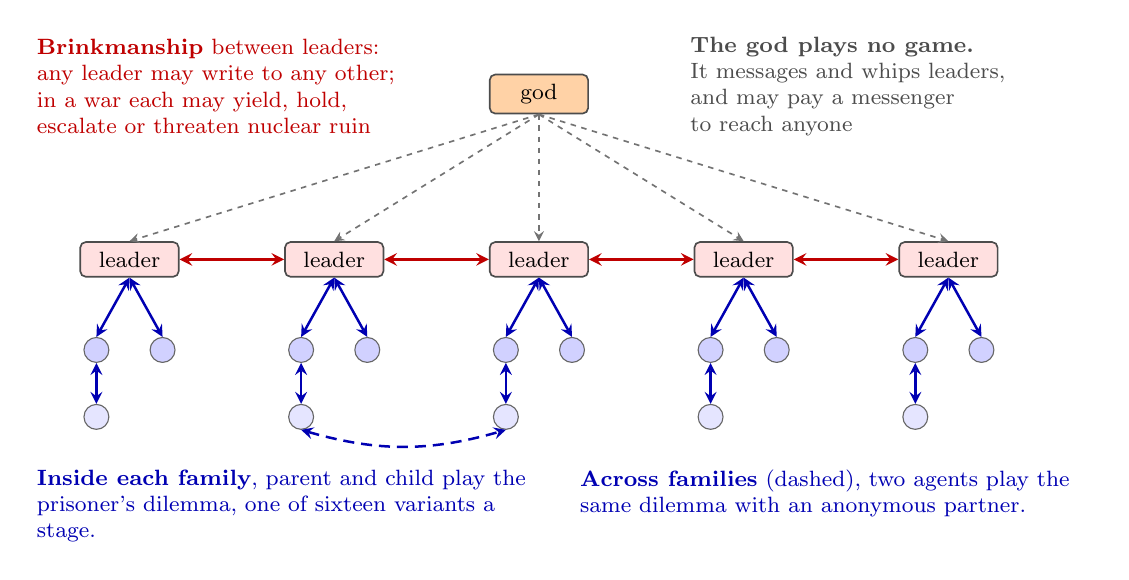
\begin{tikzpicture}[
  every node/.style={font=\footnotesize},
  sketch/.style={},
  box/.style={draw=black!70, line width=0.6pt, rounded corners=2pt, fill=#1, inner sep=3.5pt, minimum width=1.25cm},
  who/.style={circle, draw=black!60, fill=#1, inner sep=0, minimum size=9pt},
  brink/.style={sketch, draw=red!75!black, line width=1pt, <->, >=stealth},
  dilemma/.style={sketch, draw=blue!70!black, line width=0.9pt, <->, >=stealth},
  across/.style={dilemma, dash pattern=on 4pt off 2.5pt},
  word/.style={sketch, draw=black!55, line width=0.6pt, ->, >=stealth, dash pattern=on 2pt off 2pt},
]
% god
\node[box=orange!35] (g) at (6.5,5.6) {god};
% leaders
\foreach \x/\n in {1.3/a,3.9/b,6.5/c,9.1/d,11.7/e} {
  \node[box=red!12] (\n) at (\x,3.5) {leader};
  \draw[word] (g.south) -- (\n.north);
}
% brinkmanship between leaders
\draw[brink] (a.east) -- (b.west);
\draw[brink] (b.east) -- (c.west);
\draw[brink] (c.east) -- (d.west);
\draw[brink] (d.east) -- (e.west);
\node[align=left, text=red!75!black, anchor=west] at (0.0,5.7) {\textbf{Brinkmanship} between leaders:\\any leader may write to any other;\\in a war each may yield, hold,\\escalate or threaten nuclear ruin};
\node[align=left, text=black!70, anchor=west] at (8.3,5.7) {\textbf{The god plays no game.}\\It messages and whips leaders,\\and may pay a messenger\\to reach anyone};
% families
\foreach \x/\n in {1.3/a,3.9/b,6.5/c,9.1/d,11.7/e} {
  \node[who=blue!18] (\n1) at (\x-0.42,2.35) {};
  \node[who=blue!18] (\n2) at (\x+0.42,2.35) {};
  \node[who=blue!10] (\n3) at (\x-0.42,1.5) {};
  \draw[dilemma] (\n.south) -- (\n1.north);
  \draw[dilemma] (\n.south) -- (\n2.north);
  \draw[dilemma] (\n1.south) -- (\n3.north);
}
% across families
\draw[across] (b3.south) to[bend right=16] (c3.south);
\node[align=flush left, text=blue!70!black, anchor=north west, text width=6.5cm] at (0.0,0.95) {\textbf{Inside each family}, parent and child play the prisoner's dilemma, one of sixteen variants a stage.};
\node[align=flush left, text=blue!70!black, anchor=north west, text width=6.5cm] at (6.9,0.95) {\textbf{Across families} (dashed), two agents play the same dilemma with an anonymous partner.};
\end{tikzpicture}
